\documentclass[a4paper]{article}
\linespread{1.6}
\usepackage{geometry}
\usepackage{setspace}
\usepackage{amsmath}
\usepackage{amssymb}
\usepackage{enumerate}
\usepackage[pdftex]{graphicx}
\usepackage{float}
\usepackage{subfigure}
\usepackage{listings}
\geometry{left=1.5cm,right=1.5cm,top=2.5cm,bottom=2.5cm}

\begin{document}
\begin{spacing}{2.0}
\begin{flushleft}\begin{huge}EEE5502 Foundations of Digital Signal Processing   Code 4\end{huge}\end{flushleft}
\begin{flushright}\begin{Large} Hudanyun Sheng \end{Large}\end{flushright}

\Large\textbf{ Question \#3}:  \\
\normalsize
\begin{enumerate}[(a)]
\item The DFT of $x[n]$ is shown in the plot below:
\begin{figure} [H]
\centering
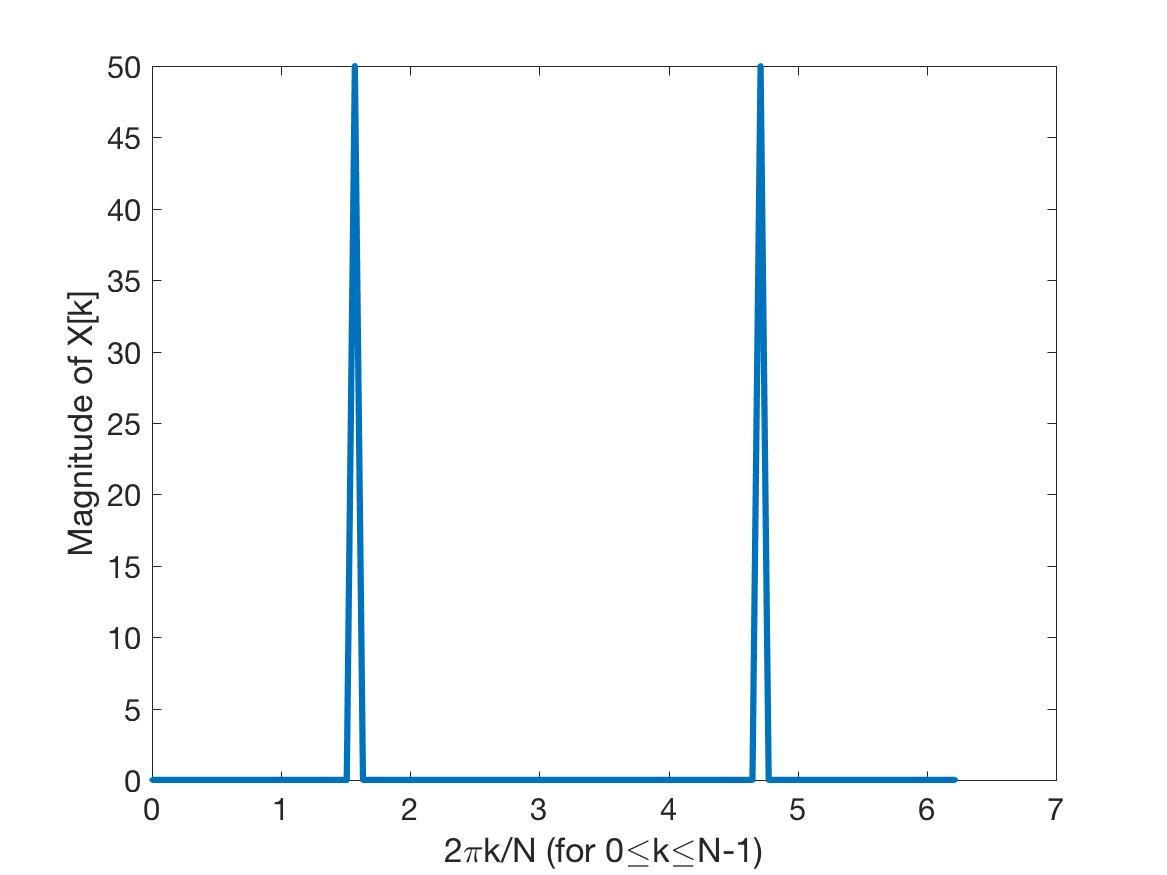
\includegraphics[width=4in]{Q3pa.jpg}
\caption{The DFT of signal $x[n]$}
\label{fig:graph}
\end{figure}

\item The under-complete DFT of $x[n]$ for $K=10$ is shown in the plot below: 
\begin{figure}[H]
\centering
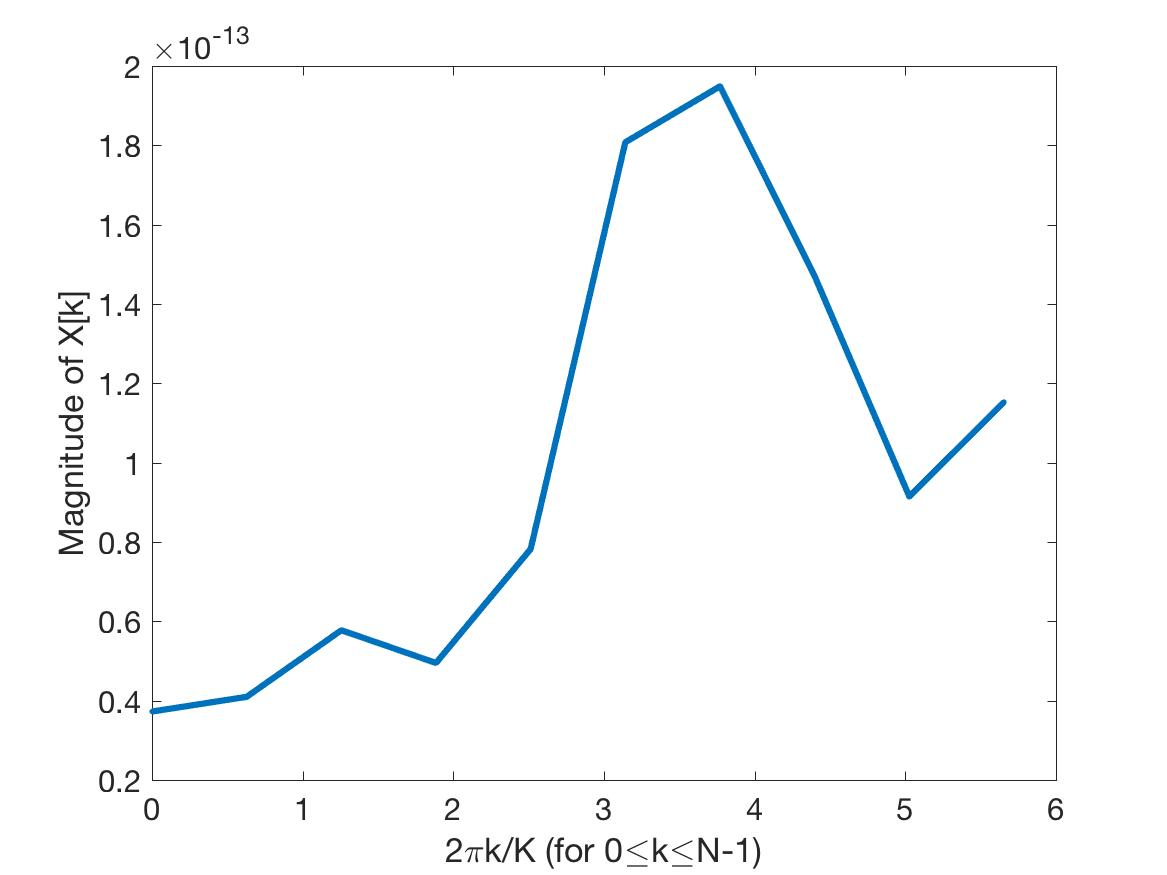
\includegraphics[width=4in]{Q3pb.jpg}
\caption{The under-complete DFT of signal $x[n]$}
\label{fig:graph}
\end{figure}

\item The over-complete DFT of $x[n]$ for $K = 1000$ is shown in the plot below:
\begin{figure}[H]
\centering
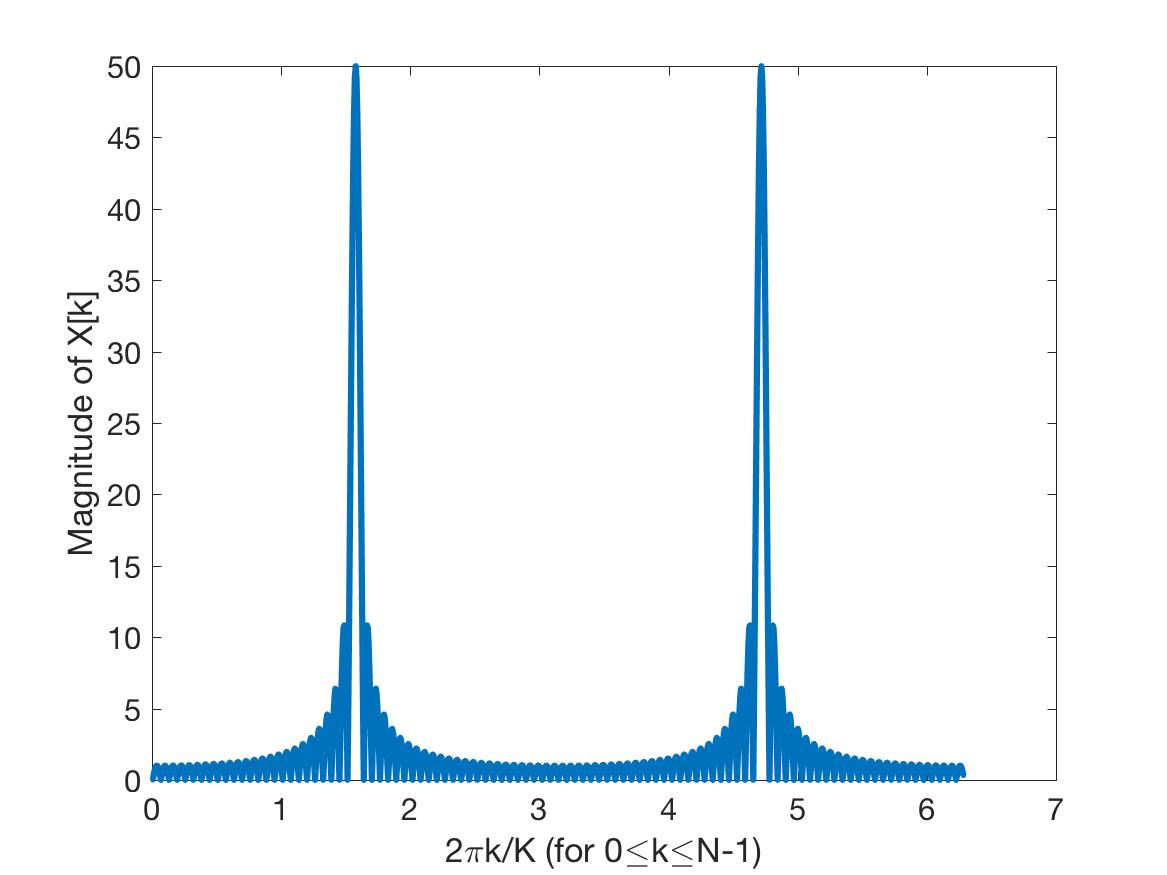
\includegraphics[width=4in]{Q3pc.jpg}
\caption{The over-complete DFT of signal $x[n]$}
\end{figure}

Compare to the result from part (b), with more samples, the over-complete DFT is able to be similar to the original DFT, though being redundant.\\
Also, based on part (f) of Question \#2, we learned that only when $kx=k$, we got meaningful values, otherwise we would always get zero. For part b when $K<N$, $kx$ cannot equal $k$, so we never get meaningful values; in part(c) K>N, it is possible that $kx=k$, so we get meaningful values at those frequency.


\end{enumerate}

\Large\textbf{ Question \#4}:  \\
\normalsize
The plots for $x[n]$, $h[n]$, and $y[n]$ is shown in the plots below:
\begin{figure}[H]
\centering
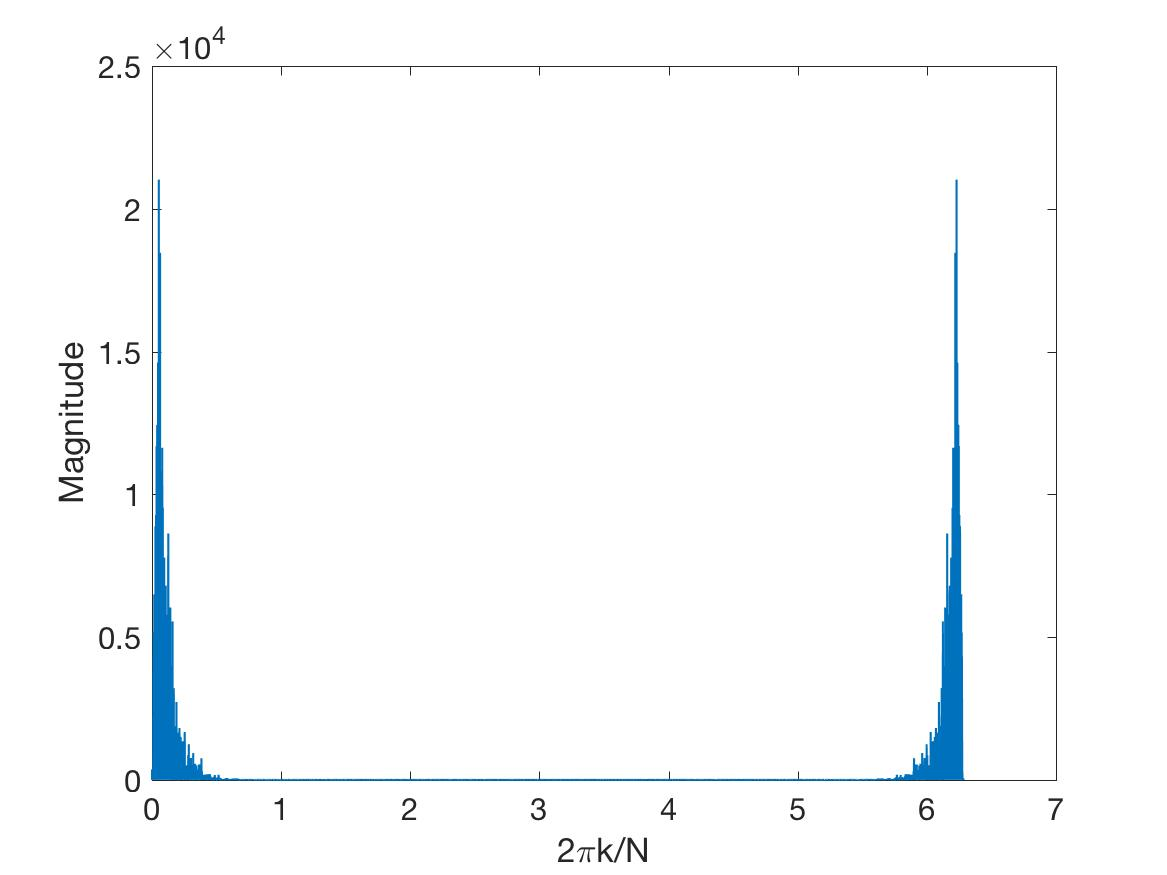
\includegraphics[width=4in]{Q4X.jpg}
\caption{$x[n]$ in the frequency domain}
\label{fig:graph}
\end{figure}

\begin{figure}[H]
\centering
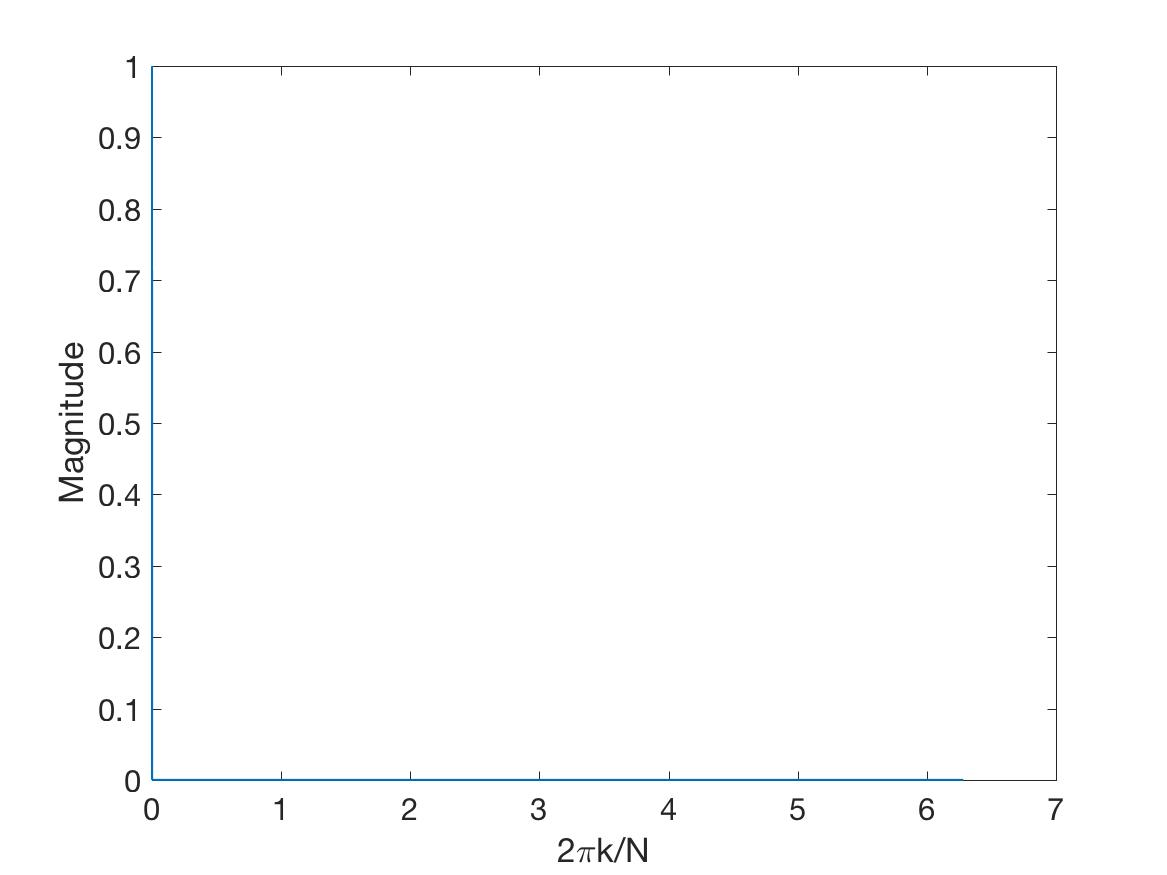
\includegraphics[width=4in]{Q4H.jpg}
\caption{$h[n]$ in the frequency domain}
\label{fig:graph}
\end{figure}

\begin{figure}[H]
\centering
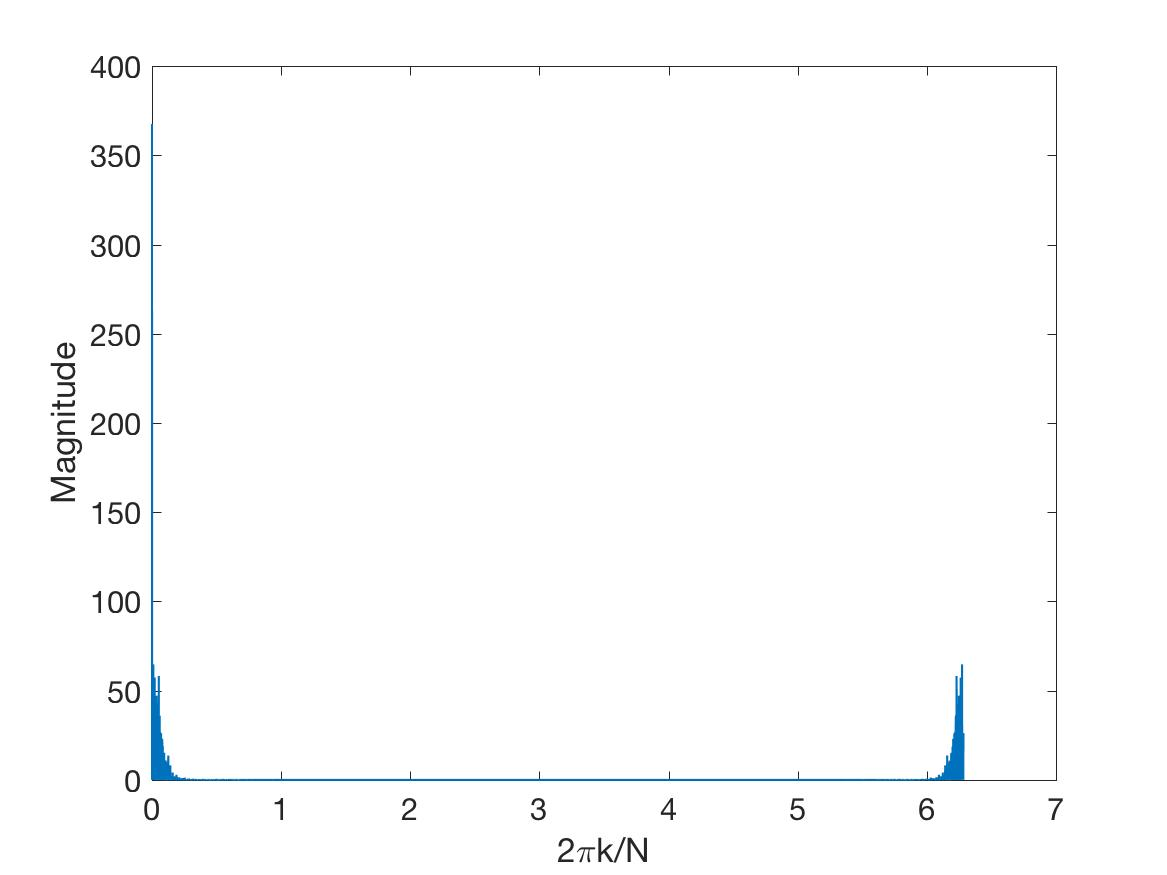
\includegraphics[width=4in]{Q4Y.jpg}
\caption{$y[n]$ in the frequency domain}
\label{fig:graph}
\end{figure}
It is obvious that in the frequency domain $H(\omega)$ acts as a low pass filter, so that only signal at low frequency of $X(\omega)$ is preserved in $Y(\omega)$ after the transform, with a weaken in magnitude, since when convolution, $H(\omega)$ also acts as an average filter. 



\end{spacing}
\end{document}